\subsubsection{Set 2 - Lindemans Aalst}
\label{sec:PL3_Aalst2}
%TODO: tekst aanpassen
Figuur \ref{fig:PL3ServeReceiveAalst2} geeft de opslag- en receptiestatistieken weer. Bij de opslag komt het teken \# overeen met 0, + en / met 1, ! met 2, - en = met 3.

De perfecte opslagen worden door beide invoermethoden gelijk geregistreed. Bij de manuele invoer bevinden zich echter geen opslagen in de categorie met score 2. De opslagen zijn daar verdeeld over score 1 en 3. Er zijn meer opslagen die score 1 hebben gekregn dan bij de AI-invoer. Bij score 3 is dit ongeveer gelijk.

De beoordeling van de receptie is op een andere wijze gedaan dan bij de manuele invoer. Bij de manuele invoer wordt er gebruik gemaakt van tekens, terwijl bij de AI-invoer gebruik wordt gemaakt van cijfers. Bij de receptie komt het teken \# overeen met 3, + en / met 2, ! met 1, - en = met 0.

De AI heeft één receptie van Max Schulz niet kunnen beoordelen. Speler Bert Dufraing heeft volgens de AI ook maar één receptie genomen, tegenover de twee die manueel zijn ingevoerd. Bij veel spelers komt de perfecte receptie bij zowel manueel als AI-invoer overeen. De andere recepties worden echter opnieuw slechter beoordeeld door de manuele invoer.

\begin{figure}[ht]
\centering
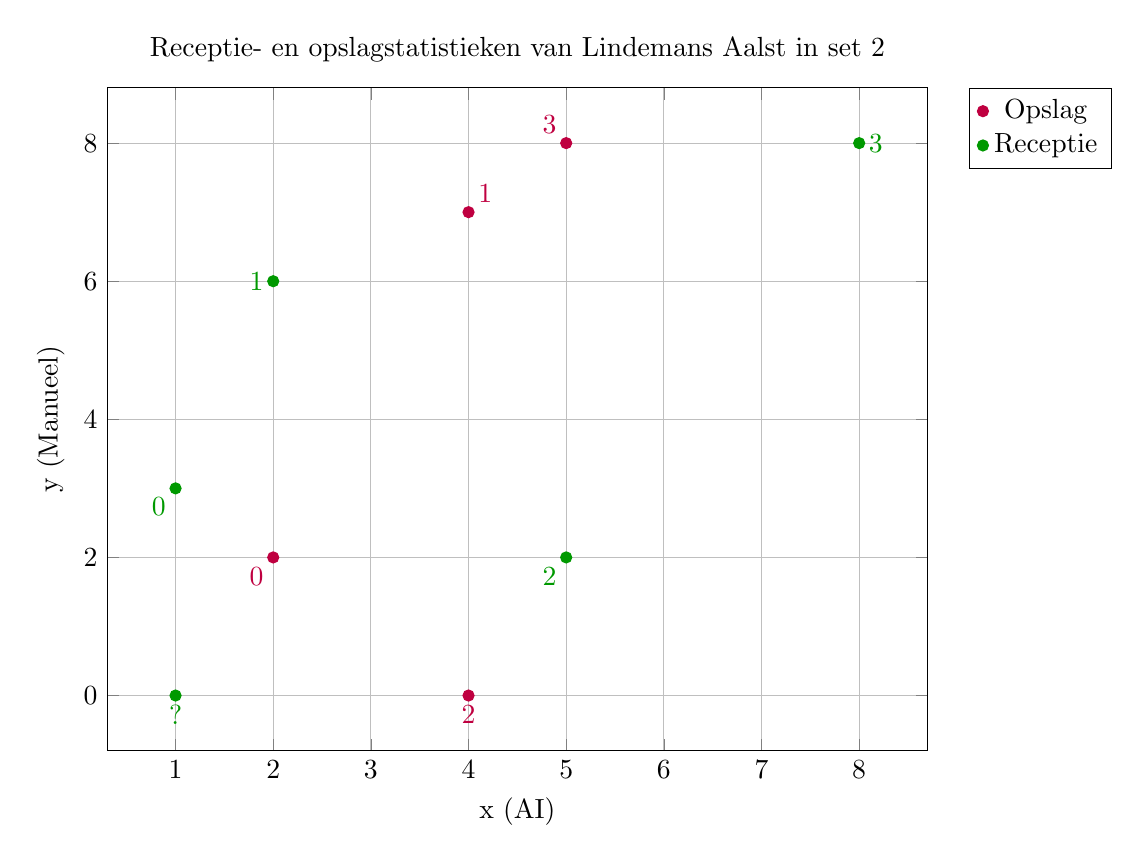
\begin{tikzpicture}
  \begin{axis}[
    title={Receptie- en opslagstatistieken van Lindemans Aalst in set 2},
    xlabel={x (AI)},
    ylabel={y (Manueel)},
    grid=major,
    legend style={at={(1.05,1)}, anchor=north west},
    width=12cm,
    height=10cm,
    enlargelimits=0.1,
  ]

  % Opslag
  \addplot[
    only marks,
    mark=*,
    color=purple,
  ] table {
    x y
    2 2
    4 7
    4 0
    5 8
  };
  \addlegendentry{Opslag}

  % Labels opslag
  \node at (axis cs:2,2) [anchor=north east, purple] {0};
  \node at (axis cs:4,7) [anchor=south west, purple] {1};
  \node at (axis cs:4,0) [anchor=north, purple] {2};
  \node at (axis cs:5,8) [anchor=south east, purple] {3};

  % Receptie
  \addplot[
    only marks,
    mark=*,
    color=green!60!black,
  ] table {
    x y
    8 8
    5 2
    2 6
    1 3
    1 0
  };
  \addlegendentry{Receptie}

  % Labels receptie
  \node at (axis cs:8,8) [anchor=west, green!60!black] {3};
  \node at (axis cs:5,2) [anchor=north east, green!60!black] {2};
  \node at (axis cs:2,6) [anchor=east, green!60!black] {1};
  \node at (axis cs:1,3) [anchor=north east, green!60!black] {0};
  \node at (axis cs:1,0) [anchor=north, green!60!black] {?};

  \end{axis}
\end{tikzpicture}
\caption{AI invoer versus manuele invoer, ingedeeld in opslag en receptie, voor Lindemans Aalst in set 2.}
\label{fig:PL3ServeReceiveAalst2}
\end{figure}

In tabel \ref{tab:PL3SetAalstMan2} en \ref{tab:PL3DigAalstMan2} zijn de manueel ingevoerde spelverdelings- en verdedigingsstatistieken weergegeven. In tabel \ref{tab:PL3SetDigAalstAI2} zijn dezelfde gegevens weergegeven die door Balltime AI zijn gemaakt.

Het aantal spelverdelingen is bij beide invoermethoden gelijk. Het aantal verdedigingsstatistieken is opnieuw minder bij de AI-invoer tegenover de manuele invoer.

\begin{table}[ht!]
    \centering
    \scriptsize
    \begin{tabular}{|l|c|c|c|c|c|c|c|c|c|}
        \hline
        \textbf{Speler} & *E\% & Tot & = & / & - & ! & + & \# \\ \hline
        Bert Dufraing & 100\% & 1 &  &  & &  & 1 & \\ 
        Lucas Lorente Lòpez & 100\% & 20 &  &  & & & 17 & 3 \\ 
        Matis Verwimp & 100\% & 1 & & & & & 1 & \\ \hline
    \end{tabular}
    \caption[Manueel ingevoerde spelverdelingsstatistieken voor Lindemans Aalst in set 2]{\label{tab:PL3SetAalstMan2}Manueel ingevoerde spelverdelingsstatistieken voor Lindemans Aalst in set 2.}
\end{table}

\begin{table}[ht!]
    \centering
    \scriptsize
    \begin{tabular}{|l|c|c|c|c|c|c|c|c|c|}
        \hline
        \textbf{Speler} & *E\% & Tot & = & / & - & ! & + & \# \\ \hline
        Bert Dufraing & 0\% & 1 & 1 &  &  &  &  & \\ 
        Timo Lohmus & 100\% & 1 &  &  &  &  & 1 & \\ 
        Berre Peters & 67\% & 3 & 1 &  &  &  & 2 & \\ 
        Alvaro Gimeno Rubio & 0\% & 2 & 2 &  &  &  &  & \\ 
        Lucas Lorente Lòpez & 0\% & 1 &  &  & 1 &  &  & \\ 
        Matis Verwimp & 0\% & 1 & 1 & & & & & \\\hline
    \end{tabular}
    \caption[Manueel ingevoerde verdedigingsstatistieken voor Lindemans Aalst in set 2]{\label{tab:PL3DigAalstMan2}Manueel ingevoerde verdedigingsstatistieken voor Lindemans Aalst in set 2.}
\end{table}

\begin{table}[ht!]
  \centering
  \scriptsize
  \begin{tabular}{|l|c|c|c|c|c|c|c|} \hline
    \textbf{Speler} & Ast & TA & SE & PCT & DS & DE \\ \hline
    Bert Dufraing &  & 1 &  & 0\% &  &  \\
    Timo Lohmus &   &   &   &   & 1  &   \\
    Berre Peters &   &   &   &   &  2 &   \\
    Alvaro Gimeno Rubio &  &  &  &  & 1 &   \\
    Lucas Lorente López & 8 & 20 &  & 40\% & 2 &  \\
    Matis Verwimp & 1 & 1 &  & 100\% &   &   \\ \hline
  \end{tabular}
  \caption[Spelverdelings- en verdedigingsstatistieken gemaakt door Balltime AI voor Lindemans Aalst in set 2]{\label{tab:PL3SetDigAalstAI2}Spelverdelings- en verdedigingsstatistieken gemaakt door Balltime AI voor Lindemans Aalst in set 2.}
\end{table}

Bij de aanvalsstatistieken (door Balltime AI in tabel \ref{tab:PL3AttBlockAalstAI2} en manuele invoer in tabel \ref{tab:PL3AttAalstMan2}) is er bij één speler een verschillend aantal aanvallen geregistreed. Hiago Crins is heeft door de AI twee keer aangevallen, terwijl hij manueel gezien maar één keer heeft aangevallen.

De blokstatistieken (door Balltime AI in tabel \ref{tab:PL3AttBlockAalstAI2} en manuele invoer in tabel \ref{tab:PL3BlockAalstMan2}) zijn ook verschillend. De AI heeft twee aanvallen geregistreerd, terwijl er manueel zes aanvallen zijn geregistreerd. 

\begin{table}[ht!]
    \centering
    \scriptsize
    \begin{tabular}{|l|c|c|c|c|c|c|c|c|c|}
        \hline
        \textbf{Speler} & *E\% & Tot & = & / & - & ! & + & \# \\ \hline
        Hiago Crins & 0\% & 1 &  &  &  & 1 &  & \\ 
        Timo Lohmus & 0\% & 5 &  & 2 & 1 &  & & 2 \\ 
        Berre Peters & 100\% & 2 &  &  & & & & 2 \\ 
        Max Schulz & -25\% & 4 &  & 1 & 1 &  & 2 & \\ 
        Alvaro Gimeno Rubio & 20\% & 5 & 1 & 1 &  &  &  & 3 \\ 
        Lou Kindt & 25\% & 4 &  &  &  &  & 3 & 1 \\
        Lucas Lorente Lòpez & 0\% & 1 &  &  &  & 1 &  & \\ \hline
    \end{tabular}
    \caption[Manueel ingevoerde aanvalsstatistieken voor Lindemans Aalst in set 2]{\label{tab:PL3AttAalstMan2}Manueel ingevoerde aanvalsstatistieken voor Lindemans Aalst in set 2.}
\end{table}

\begin{table}[ht!]
    \centering
    \scriptsize
    \begin{tabular}{|l|c|c|c|c|c|c|c|c|c|}
        \hline
        \textbf{Speler} & *E\% & Tot & = & / & - & ! & + & \# \\ \hline
        Hiago Crins & -50\% & 2 & 1 &  &  &  & 1 &  \\
        Max Schulz & -100\% & 1 & 1 &  &  &  &  & \\
        Mihkel Varblane & -50\% & 2 & 1 &  &  & 1 &  & \\
        Lou Kindt & -100\% & 1 & 1 &  &  &  &  & \\
        Lucas Lorente Lòpez & 0\% & 1 &  &  &  &  & 1 & \\ \hline
    \end{tabular}
    \caption[Manueel ingevoerde blokstatistieken voor Lindemans Aalst in set 2]{\label{tab:PL3BlockAalstMan2}Manueel ingevoerde blokstatistieken voor Lindemans Aalst in set 2.}
\end{table}

\begin{table}[ht!]
  \centering
  \scriptsize
  \begin{tabular}{|l|c|c|c|c|c|c|c|c|c|c|c|} \hline
    \textbf{Speler} &  K & E & TA & Atk\% & Kill\% & Error\% & BS & BA & BE \\ \hline
    Hiago Crins &  &  & 2 & 0.00 & 0\% & 0\% &  &  &\\
    Timo Lohmus & 2 & 2 & 5 & 0.0 & 40\% & 40 \%&  & 1 & \\
    Berre Peters & 2 &  & 2 & 1.00 & 100\% & 0\% &   &  & \\
    Max Schulz & 1 &  & 4 & 0.25 & 25\% & 0\% &   &  & \\
    Mihkel Varblane &   &   &   &   &   &   &  & 1 &\\
    Alvaro Gimeno Rubio & 3 & 2 & 5 & 0.20 & 60\% & 40\% &   &  & \\
    Lou Kindt & 1 &  & 4 & 0.25 & 25\% & 0\% &   &  & \\ \hline
  \end{tabular}
  \caption[Aanvals- en blokstatistieken gemaakt door Balltime AI voor Lindemans Aalst in set 2]{\label{tab:PL3AttBlockAalstAI2}Aanvals- en blokstatistieken gemaakt door Balltime AI voor Lindemans Aalst in set 2.}
\end{table}
